\documentclass[10pt,a4paper]{article}

\usepackage[utf8]{inputenc}
\usepackage[T1]{fontenc}
\usepackage[italian]{babel}
\usepackage{amsmath,amssymb}
\usepackage{multicol}
\usepackage{geometry}
\usepackage{enumitem}
\usepackage{xcolor}
\usepackage{pdfpages}
\usepackage{tabularx} % <-- Aggiunto per la formattazione della tabella
\usepackage{graphicx}

% Margini stretti per far stare il formulario in mezza pagina A4
\geometry{a4paper,left=0.5cm,right=0.5cm,top=0.5cm,bottom=0.5cm}

% Spaziatura compatta
\setlength{\parindent}{0pt}
\setlength{\parskip}{0pt}
\setlength{\abovedisplayskip}{0pt}
\setlength{\belowdisplayskip}{0pt}
\setlength{\abovedisplayshortskip}{0pt}
\setlength{\belowdisplayshortskip}{0pt}
\setlength{\columnsep}{12pt}

% Comando per i titoletti delle sotto-sezioni
\newcommand{\sub}[1]{\smallskip\noindent\textbf{#1}\par\nobreak}

\begin{document}

\centerline{\textbf{\large Formulario Prima Parte}}
\vspace{-1mm}

\begin{center}
\fbox{\parbox{0.97\textwidth}{%
\footnotesize
\begin{minipage}[t]{0.48\textwidth}
\vspace{0pt}
\centerline{\textbf{\underline{Soluzioni delle equazioni di stato}}}
\vspace{4pt}

{\centering $x(t) = x_{zi}(t) + x_{zs}(t) \quad x(k) = x_{zi}(k) + x_{zs}(k)$\par}

\vspace{4pt}
\renewcommand{\arraystretch}{1.4}
\begin{tabularx}{\linewidth}{|>{\centering\arraybackslash}X|>{\centering\arraybackslash}X|}
\hline
$X_{zi}(s) = (sI - A)^{-1}x(0)$ & $X_{zs}(s) = (sI - A)^{-1}BU(s)$ \\
\hline
$X_{zi}(z) = z(zI - A)^{-1}x(0)$ & $X_{zs}(z) = (zI - A)^{-1}BU(z)$ \\
\hline
\multicolumn{2}{|c|}{$y(t) = y_{zi}(t) + y_{zs}(t) \quad y(k) = y_{zi}(k) + y_{zs}(k)$} \\
\hline
$Y_{zi}(s) = C(sI - A)^{-1}x(0)$ & $Y_{zs}(s) = H(s)U(s)$ \\
\hline
$Y_{zi}(z) = C z(zI - A)^{-1}x(0)$ & $Y_{zs}(z) = H(z)U(z)$ \\
\hline
\end{tabularx}
\end{minipage}%
\hfill
\begin{minipage}[t]{0.48\textwidth}
\vspace{0pt}
\centerline{\textbf{\underline{formule utili}}}
\vspace{4pt}

\renewcommand{\arraystretch}{1.6}
\begin{tabularx}{\linewidth}{|>{\centering\arraybackslash}X|>{\centering\arraybackslash}X|}
\hline
contributo poli complessi e coniugati (TC) \newline $2|R|e^{Re(p_i)t} \cdot \cos(Im(p_i)t + \angle R)$ & 
$\mathcal{L}\left\{ \frac{t^n e^{-\lambda t}}{n!} \right\} = \frac{1}{(s + \lambda)^{n+1}}$ \\
\hline
contributo poli complessi e coniugati (TD) \newline $2|R||a|^k \cdot \cos(\angle a\, k + \angle R)$ & 
$\mathcal{L}\{\dot{f}(t)\} = sF(s) - f(0)$ \\
\hline
$\mathcal{Z}\{a^k\} = \frac{z}{z-a}, \quad \tilde{F}(z) = \frac{F(z)}{z}$ & 
$\mathcal{Z}\{f(k+1)\} = zF(z) - zf(0)$ \\
\hline
$\tau_i = \left| \frac{1}{Re(p_i)} \right|$ (costanti di tempo poli) & 
$\mathcal{L}\{\varepsilon(t)\} = \frac{1}{s} \newline \mathcal{Z}\{\varepsilon(t)\} = \frac{z}{z-1}$ \\
\hline
\end{tabularx}
\end{minipage}
}}
\end{center}

\vspace{-1.5mm}

\begin{center}
\fbox{\parbox{0.97\textwidth}{%
\footnotesize
\noindent\textbf{\underline{Stabilità}} \quad $Spec(A) = \{\lambda_i \in \mathbb{C} \mid p_A(\lambda_i) = 0\}$=autovalori A \quad e = \texttt{eig(A)}; \texttt{[V, D]=eig(A)}

\vspace{-2pt}
\begin{minipage}{0.83\textwidth}
\renewcommand{\arraystretch}{1.2}
\begin{tabularx}{\textwidth}{|>{\itshape}p{2.3cm}|X|X|}
\hline
& \textbf{TEMPO CONTINUO} (vedi Criterio di Routh) & \textbf{TEMPO DISCRETO} (vedi Criterio di Jury) \\
\hline
asintoticamente \newline stabile & 
\parbox[t]{0.45\linewidth}{$\forall x_0 \in \mathbb{R}^n,$\\$x_{zi}(t)$ limitata} \hfill
\parbox[t]{0.45\linewidth}{$Re(\lambda_i) < 0 \; \forall i$} & 
\parbox[t]{0.45\linewidth}{$\forall x_0 \in \mathbb{R}^n,$\\$x_{zi}(k)$ limitata} \hfill
\parbox[t]{0.45\linewidth}{$|\lambda_i| < 1 \; \forall i$} \\
\hline
internamente \newline stabile & 
\parbox[t]{0.45\linewidth}{$\forall x_0 \in \mathbb{R}^n,$\\$x_{zi}(t)$ limitata\\$\lim_{t\to\infty} x_{zi}(t) \neq 0$} \hfill
\parbox[t]{0.45\linewidth}{$Re(\lambda_i) \leq 0 \; \forall i$\\$Re(\lambda_i) = 0, \mu_g = \mu_a$} & 
\parbox[t]{0.45\linewidth}{$\forall x_0 \in \mathbb{R}^n,$\\$x_{zi}(k)$ limitata\\$\lim_{k\to\infty} x_{zi}(k) \neq 0$} \hfill
\parbox[t]{0.45\linewidth}{$|\lambda_i| \leq 1 \; \forall i$\\$|\lambda_i| = 1, \mu_g = \mu_a$} \\
\hline
BIBO stabile & 
\parbox[t]{0.45\linewidth}{$x_0 = 0$\\$\forall u(t)$ limitato\\$y_{zs}(t)$ limitato} \hfill
\parbox[t]{0.45\linewidth}{$Re(p_i) < 0 \; \forall i$\\$p_i$ poli del sistema} & 
\parbox[t]{0.45\linewidth}{$x_0 = 0$\\$\forall u(k)$ limitato\\$y_{zs}(k)$ limitato} \hfill
\parbox[t]{0.45\linewidth}{$|p_i| < 1 \; \forall i$\\$p_i$ poli del sistema} \\
\hline
instabile & 
\parbox[t]{0.45\linewidth}{$\exists x_0 \in \mathbb{R}^n,$\\$x_{zi}(t)$ illimitata} \hfill
\parbox[t]{0.45\linewidth}{$\exists \lambda_i \mid Re(\lambda_i) > 0 $\\$\exists \lambda_i \mid Re(\lambda_i) = 0,$\\$\mu_g > 1$} & 
\parbox[t]{0.45\linewidth}{$\exists x_0 \in \mathbb{R}^n,$\\$x_{zi}(k)$ illimitata} \hfill
\parbox[t]{0.45\linewidth}{$\exists \lambda_i \mid |\lambda_i| > 1 $\\$\exists \lambda_i \mid |\lambda_i| = 1,$\\$\mu_g > 1$} \\
\hline
\end{tabularx}
\end{minipage}

\vspace{4pt}
\textbf{Nota:} Molteplicità geometrica \quad $m_g(\lambda_0) = \text{rank}(A) - \text{rank}(A - \lambda_0 I_n)$
}}
\end{center}

\vspace{-1.5mm}

\begin{center}
\fbox{\parbox{0.97\textwidth}{%
\footnotesize
\textbf{\underline{Linearizzazione di sistemi non LTI}}
\vspace{2pt}

\sub{Calcolo punti di equilibrio}
\vspace{-2pt}
\[
\begin{cases} \dot{x} = f(x,u) \\ y = g(x,u) \end{cases} \rightarrow
\begin{cases} \dot{x}_1 = f_1(x,u) \\ \dot{x}_2 = f_2(x,u) \end{cases} \xrightarrow[\text{derivate a zero}]{\text{impongo}}
\begin{cases} f_1(x,u) = 0 \\ f_2(x,u) = 0 \end{cases} \Rightarrow
\bar{x} = [\bar{x}_1\ \ \bar{x}_2\ \ \dots]
\]

\sub{Linearizzazione}
\vspace{-2pt}
\[
\begin{cases} \delta\dot{x}(t) = A\delta x(t) + B\delta u(t) \\ \delta y(t) = C\delta x(t) + D\delta u(t) \end{cases}
\]
\vspace{2pt}

\renewcommand{\arraystretch}{1.5}
\begin{tabularx}{\linewidth}{>{\centering\arraybackslash}X>{\centering\arraybackslash}X}
$ A = \frac{\partial f(x,u)}{\partial x} \bigg|_{\substack{x=\bar{x}\\u=\bar{u}}} \hspace{-2mm} = \begin{bmatrix} \partial f_1/\partial x_1 & \dots & \partial f_1/\partial x_n \\ \vdots & \ddots & \vdots \\ \partial f_n/\partial x_1 & \dots & \partial f_n/\partial x_n \end{bmatrix}_{\substack{x=\bar{x}\\u=\bar{u}}} $ &
$ C = \frac{\partial g(x,u)}{\partial x} \bigg|_{\substack{x=\bar{x}\\u=\bar{u}}} \hspace{-2mm} = \begin{bmatrix} \partial g_1/\partial x_1 & \dots & \partial g_1/\partial x_n \\ \vdots & \ddots & \vdots \\ \partial g_q/\partial x_1 & \dots & \partial g_q/\partial x_n \end{bmatrix}_{\substack{x=\bar{x}\\u=\bar{u}}} $ \\
$ B = \frac{\partial f(x,u)}{\partial u} \bigg|_{\substack{x=\bar{x}\\u=\bar{u}}} \hspace{-2mm} = \begin{bmatrix} \partial f_1/\partial u_1 & \dots & \partial f_1/\partial u_p \\ \vdots & \ddots & \vdots \\ \partial f_n/\partial u_1 & \dots & \partial f_n/\partial u_p \end{bmatrix}_{\substack{x=\bar{x}\\u=\bar{u}}} $ &
$ D = \frac{\partial g(x,u)}{\partial u} \bigg|_{\substack{x=\bar{x}\\u=\bar{u}}} \hspace{-2mm} = \begin{bmatrix} \partial g_1/\partial u_1 & \dots & \partial g_1/\partial u_p \\ \vdots & \ddots & \vdots \\ \partial g_q/\partial u_1 & \dots & \partial g_q/\partial u_p \end{bmatrix}_{\substack{x=\bar{x}\\u=\bar{u}}} $ \\
\end{tabularx}
}}
\end{center}

\vspace{-1.5mm}

\begin{center}
\makebox[\dimexpr 0.97\textwidth + 2\fboxsep + 2\fboxrule\relax][s]{%
\fbox{\parbox[t]{0.64\textwidth}{%
\footnotesize
\textbf{\underline{Controllabilità e retroazione statica dello stato}}
\vspace{2pt}

\textbf{1)} Voglio assegnare a $(A-BK)$ gli autovalori scelti da me nel vettore $\lambda = [\lambda_1\ \lambda_2\ \dots\ \lambda_n]$.\\
\textbf{2)} Verifico se il problema può essere risolto:
\vspace{-4pt}
\[
M_R = \mathtt{ctrb}(A,B), \quad r = \mathtt{rank}(M_R), \quad r \begin{cases} = n \Rightarrow \text{OK, posso risolvere} \\ < n \Rightarrow \text{NO, non ha soluzione} \end{cases}
\]
\vspace{-4pt}

\textbf{3)} Posso calcolare $K$ t.c. $\mathtt{eig}(A-BK) = \lambda$ usando:
\begin{itemize}[leftmargin=15pt, nosep, before=\vspace{-2pt}, after=\vspace{-2pt}]
    \item $K = \mathtt{place}(A, B, \lambda) \Rightarrow$ non permette di assegnare tutti autovalori identici
    \item oppure $K = \mathtt{acker}(A, B, \lambda) \Rightarrow$ numericamente più ``fragile''
\end{itemize}
\vspace{2pt}
\textbf{4)} Nuovo sistema: $\begin{cases} \dot{x} = (A-BK)x + B\alpha u \\ y(t) = Cx(t) + Du(t) \end{cases}$
}}%
\hfill
\fbox{\parbox[t]{0.31\textwidth}{%
\footnotesize
\textbf{\underline{Stabilità del sistema linearizzato}}
\vspace{2pt}

\renewcommand{\arraystretch}{1.5}
\begin{tabularx}{\linewidth}{|>{\centering\arraybackslash}X|>{\centering\arraybackslash}X|}
\hline
\textbf{Autovalori $\lambda_i(A)$} & \textbf{Stabilità} \\
\hline
$\forall i : Re(\lambda_i(A)) < 0$ & \textbf{Asintoticamente stabile} \\
\hline
$\exists i : Re(\lambda_i(A)) > 0$ & \textbf{Instabile} \\
\hline
$\forall i : Re(\lambda_i(A)) \le 0$ & \textbf{Nessuna conclusione} \\
\hline
\end{tabularx}
}}%
}
\end{center}

\vspace{-1.5mm}

\begin{center}
\fbox{\parbox{0.97\textwidth}{%
\footnotesize
\textbf{\underline{Osservabilità e Progetto dell'osservatore}}
\vspace{2pt}

\textbf{Verifica Osservabilità:}\quad $M_o = \mathtt{obsv}(A,C) \rightarrow \text{se } \mathtt{rank}(M_o) = n \quad \text{sistema completamente osservabile}$

\vspace{2pt}
\textbf{Progetto osservatore:}\quad $L = (\mathtt{place}(A', C', \lambda_{des}))'$

\vspace{2pt}
\textbf{Modello dell'osservatore:} \quad
$\begin{cases}
\dot{\hat{x}} = A\hat{x}(t) + Bu(t) - L(\hat{y}(t) - y(t)) \\
\hat{y}(t) = C\hat{x}(t) + Du(t)
\end{cases}$
}}
\end{center}

\newpage

\centerline{\textbf{\large Formulario Seconda Parte}}
\vspace{-1mm}

\begin{center}
\fbox{\parbox{0.97\textwidth}{%
\begin{center}\textbf{\large 1) Determinazione specifiche di progetto}\end{center}
\vspace{-4pt}
\footnotesize
\textbf{Incognite:} $G_F$;
$K_c$ da $\varepsilon_r$; $K_c$ da $d_a$ e/o $d_p$; $\omega_c$ da $d_p$ e/o $d_s$; $\zeta,\,T_{p,0},\,S_{p,0}$ da $\hat{s}$; $\omega_c$ da $t_r$;
$\omega_c$ da $t_{s,\varepsilon\%}$; \;$\nu$ da $d_a$ e/o $d_p$; \;$M_S^{LF}$, $M_T^{HF}$.
\begin{multicols}{2}

\sub{a) Calcolo $G_F$}
\[
G_F=\frac{1}{G_s\,K_d} \quad \text{se } \nu+p>0
\]

\sub{b) Calcolo $\nu$ e $K_c$ da $\varepsilon_r$}
se $\varepsilon_r=0 \rightarrow \nu>h-p, |K_c|=\forall$\\
se $\varepsilon_r\neq 0 \rightarrow \nu = h-p$ \;\;
\[
|K_c|\geq
\begin{cases}
\left|\dfrac{R_0\,K_d^{2}}{\varepsilon_r\,K_p\,G_a}\right| & \text{se } \nu+p\neq 0\\[10pt]
\dfrac{\dfrac{R_0\,K_d^{2}}{\varepsilon_r}-K_d}{K_p\,G_a} & \text{se } \nu+p=0
\end{cases}
\]
$K_p$ = guadagno di $G_p$ in cost.\ tempo.
($p$: poli nell'origine di $G_p$ espresso in cost.\ tempo)
\vspace{2pt}
{\scriptsize
\[
\mathtt{zpk\_gp = zpk(Gp);}
\]
\vspace{-4pt}
\[
\mathtt{zpk(zpk\_gp.Z, zpk\_gp.P, zpk\_gp.K, \text{`DisplayFormat'}, \text{`timeconstant'})}
\]
}

\sub{c) Calcolo $K_c$ da $d_a$}
\[
|e_{\infty}^{d_a}|
= \left|\lim_{t\to\infty} e_{d_a}(t)\right| = \left|\lim_{t\to\infty} y_{d_a}(t)\right| = \left|\lim_{s\to 0} s\, G_{d_a y}(s)\, d_a(s)\right|
\]
\[
|K_c|\geq\left|\frac{D_{a,0}}{\varepsilon_{d_a}\,G_a\,G_s\,G_F}\right|\quad\text{se } \varepsilon_{d_a}\neq 0\ \Rightarrow\ \nu = h_a
\]
\[
|K_c|=\forall\quad\text{se } \varepsilon_{d_a}=0\ \Rightarrow\ \nu>h_a
\]

\noindent\begin{minipage}{\columnwidth}
\sub{d) Calcolo $K_c$ da $d_p$ (polinomiale) o $\omega_c/M_S^{LF}$ (sinusoidale)}
\emph{Polinomiale:}
\[
|e_{\infty}^{d_p}|
= \left|\lim_{t\to\infty} e_{d_p}(t)\right| = \left|\lim_{t\to\infty} y_{d_p}(t)\right| = \left|\lim_{s\to 0} s\, G_{d_p y}(s)\, d_p(s)\right|
\]
\[
|K_c|\geq\left|\frac{D_{p,0}}{\varepsilon_{d_p}\,G_a\,G_s\,G_F\,K_p}\right|\quad\text{se } \varepsilon_{d_p}\neq 0\ \Rightarrow\ \nu = h_p-p
\]
\[
|K_c|=\forall\quad\text{se } \varepsilon_{d_p}=0\ \Rightarrow\ \nu>h_p-p
\]
\end{minipage}
\begin{minipage}{\columnwidth}
\emph{Sinusoidale:}
\[
|e_{\infty}^{d_p}| = \left|G_{d_p y}(j\omega_p) a_p \sin(\omega t + \varphi_p)\right|
\leq |S(j\omega_p)|\
\]
\[
M_S^{LF}=\frac{\rho_p}{a_p},\qquad M_{S,\,dB}^{LF}=20\log_{10}M_S^{LF}
\]
\[
\omega_L=\omega_p\cdot 10^{-\,M_{S,\,dB}^{LF}/40},\qquad \omega_c\geq 2\,\omega_L
\]
\end{minipage}

\sub{e) Calcolo $\omega_c/M_T^{HF}$ da $d_s$ (sinusoidale)}
\[
|e_{\infty}^{d_s}| = \left|G_{d_s y}(j\omega_s) a_s \sin(\omega t + \varphi_s)\right|
\leq |T(j\omega_s)|\
\]
\[
M_T^{HF}=\frac{\rho_s\,G_s}{a_s},\qquad M_{T,\,dB}^{HF}=20\log_{10}M_T^{HF}
\]
\[
\omega_H=\omega_s\cdot 10^{\,M_{T,\,dB}^{HF}/40},\qquad \omega_c\leq\frac{\omega_H}{2}
\]

\sub{f) Calcolo $\zeta,\,T_{p,0},\,S_{p,0}$ da $\hat{s}$}
\[
\zeta\ge\frac{|\ln(\hat{s})|}{\sqrt{\pi^{2}+\ln^{2}(\hat{s})}}
\]
\[
T_{p,0}\leq\frac{1}{2\zeta\sqrt{1-\zeta^{2}}}
\]
\[
S_{p,0}\leq\frac{2\zeta\sqrt{2+4\zeta^{2}+2\sqrt{1+8\zeta^{2}}}}{\sqrt{1+8\zeta^{2}}+4\zeta^{2}-1}
\]

\sub{g) Calcolo $\omega_c$ da $t_r$ e $\varepsilon_{s,\%}$}
\[
t_r:\quad \omega_c\geq\left(\frac{\pi-\arccos(\zeta)}{t_r\sqrt{1-\zeta^{2}}}\right)\sqrt{\sqrt{1+4\zeta^{4}}-2\zeta^{2}}
\]
\[
t_{s,\alpha\%}:\ \omega_c\geq\left(\frac{|\ln(\alpha\%)|}{\zeta\,t_{s,\alpha\%}}\right)\sqrt{\sqrt{1+4\zeta^{4}}-2\zeta^{2}}
\]

\sub{h) Conclusioni}
Scelgo $\nu$ più grande tra i $\nu$ che ho trovato e prendo il $K_c$ più grande tra quelli che ho trovato \underline{con quel $\nu$}.
\end{multicols}
}}
\end{center}

\vspace{-1.5mm} % <-- Spazio ulteriormente compattato

\begin{center}
\fbox{\parbox{0.97\textwidth}{%
\begin{center}\textbf{\large 2) Progetto del Sistema di Controllo}\end{center}
\vspace{-4pt}
\footnotesize

\begin{multicols}{2}

\noindent\begin{minipage}{\columnwidth}
\sub{Passo 1: Studio del segno di $K_c$ e stabilizzabilità}
a.
Scelgo un segno e calcolo $L_{in}(s)$:
\[
L_{in}(s) = \frac{K_c}{s^\nu} \cdot G_F \, G_a \, G_p \, G_s
\]
b.
Tracciare il diagramma di Nyquist di $L_{in}(s)$ e calcolo \\ $P_{cl}=N+P_{ol}$, dove:\\
\hspace*{3mm} $N$: intersezioni semiretta\\
\hspace*{3mm} $P_{ol}$: poli con $Re(p_i) > 0$ (di solito nullo)
\begin{itemize}[leftmargin=*, nosep, before=\vspace{-2pt}, after=\vspace{-2pt}]
    \item $P_{cl}$ pari $\rightarrow$ \textbf{Stabilizzabile}
    \item $P_{cl}$ dispari $\rightarrow$ \textbf{Cambio segno di $K_c$}
\end{itemize}
c.
Scelgo $K_c$ poco più grande del vincolo (se c'è).

\vspace{2pt}
{\scriptsize
\[
[N_{L_{in}}, D_{L_{in}}] = \mathtt{tfdata}(L_{in}, \text{``v''})
\]
\[
\mathtt{myngridst}(T_{p,0}, S_{p,0})
\]
\[
\mathtt{nyquist1}(N_{L_{in}}, D_{L_{in}})
\]
}
\end{minipage}

\noindent\begin{minipage}{\columnwidth}
\sub{Passo 2: Reti di compensazione}
Plot di $L_{in}(s)$ sul piano di Nichols e individuo $\omega_{c,des}$ scegliendo l'azione con le \textbf{reti di compensazione} per:

\sub{Passo 3: Simulazione}
Simulare con \texttt{step(T/(Gs*Gf))} per le specifiche in transitorio. Se $\hat{s}$ non rispettato aumento provo ad aumentare $\omega_{norm}$, se $t_{s,\alpha\%}$ non rispettato aumento provo ad aumentare $\omega_{des}$. (Le altre su inseguimento e disturbi sono verificate se $K_c$ e $\nu$ sono OK).

\sub{Passo 4: Verifica Bode di T ed S}
Verificare che i diagrammi stiano sotto i relativi spigoli.
\begin{itemize}[leftmargin=12pt, nosep, before=\vspace{-2pt}, after=\vspace{-2pt}]
    \item[a.] Taglia spigolo \textbf{T}? $\rightarrow$ aggiungo un polo $(1 + s/\omega_s)^{-1}$
    \item[b.] Taglia spigolo \textbf{S}? $\rightarrow$ Alzo $K_c$
\end{itemize}
\vspace{2pt}
\textbf{Nota}: $S(s) = \frac{1}{1+L}, \quad T(s) = \frac{L}{1+L}$
\end{minipage}

\end{multicols}
}}
\end{center}

\vspace{-1.5mm} % <-- Spazio ulteriormente compattato

% --- NUOVA TABELLA DELLE RETI DI COMPENSAZIONE ---
\begin{center}
\fbox{\parbox{0.97\textwidth}{%
\centerline{\textbf{3) Principali reti di compensazione}}
\vspace{2pt}
\footnotesize
\renewcommand{\arraystretch}{1.4} % Allarga un po' le righe per le frazioni
\begin{tabularx}{\linewidth}{|>{\raggedright\arraybackslash}X|>{\raggedright\arraybackslash}p{2.6cm}|>{\raggedright\arraybackslash}p{3cm}|>{\raggedright\arraybackslash}p{4.8cm}|}
\hline
\textbf{\textit{Soluzione}} & \textbf{\textit{Formule utili}} & \textbf{\textit{Alternativa}} & \\
\hline
\textbf{\underline{Rete LEAD}}\newline aumento di modulo\newline aumento di fase\newline $R_d(s) = \dfrac{1 + \frac{s}{z_d}}{1 + \frac{s}{m_d z_d}}, m_d > 1$ 
& $z_d = \dfrac{\omega_{cdes}}{\omega_{norm}}$ 
& \textbf{\underline{Rete ZERO}}\newline aumento di modulo\newline aumento di fase\newline $R_z(s) = \left(1 + \frac{s}{z}\right)$
& Da usare solo nel caso in cui $\nu > 0$ (posso mettere al massimo $\nu$ reti zero) (Da preferire sempre alla rete LEAD)\\
\hline
\textbf{\underline{Rete LAG}}\newline diminuzione modulo\newline $R_i(s) = \dfrac{1 + \frac{s}{m_i p_i}}{1 + \frac{s}{p_i}}, m_i > 1$ 
& $m_i = 10^{\frac{R_{db}}{20}}$\newline \newline $p_i = \dfrac{\omega_{cdes}}{\omega_{norm}}$ 
& \underline{Diminuzione di $|K_c|$}\newline \mbox{$K_c = K_{c,in} 10^{\frac{-|K_{c,dB}^{sub}|}{20}}$}
& Solo quando ho $K_c$ libero ($|K_c| = 1$) o se ho scelto $K_c$ maggiore del vincolo (fare attenzione a non fare scendere il nuovo $K_c$ sotto al vincolo) \\
\hline
\underline{Aumento di $|K_c|$}\newline aumento di modulo 
& \mbox{$K_c = K_{c,in} 10^{\frac{|K_{c,dB}^{add}|}{20}}$}
& 
& \\
\hline
\end{tabularx}
}}
\end{center}

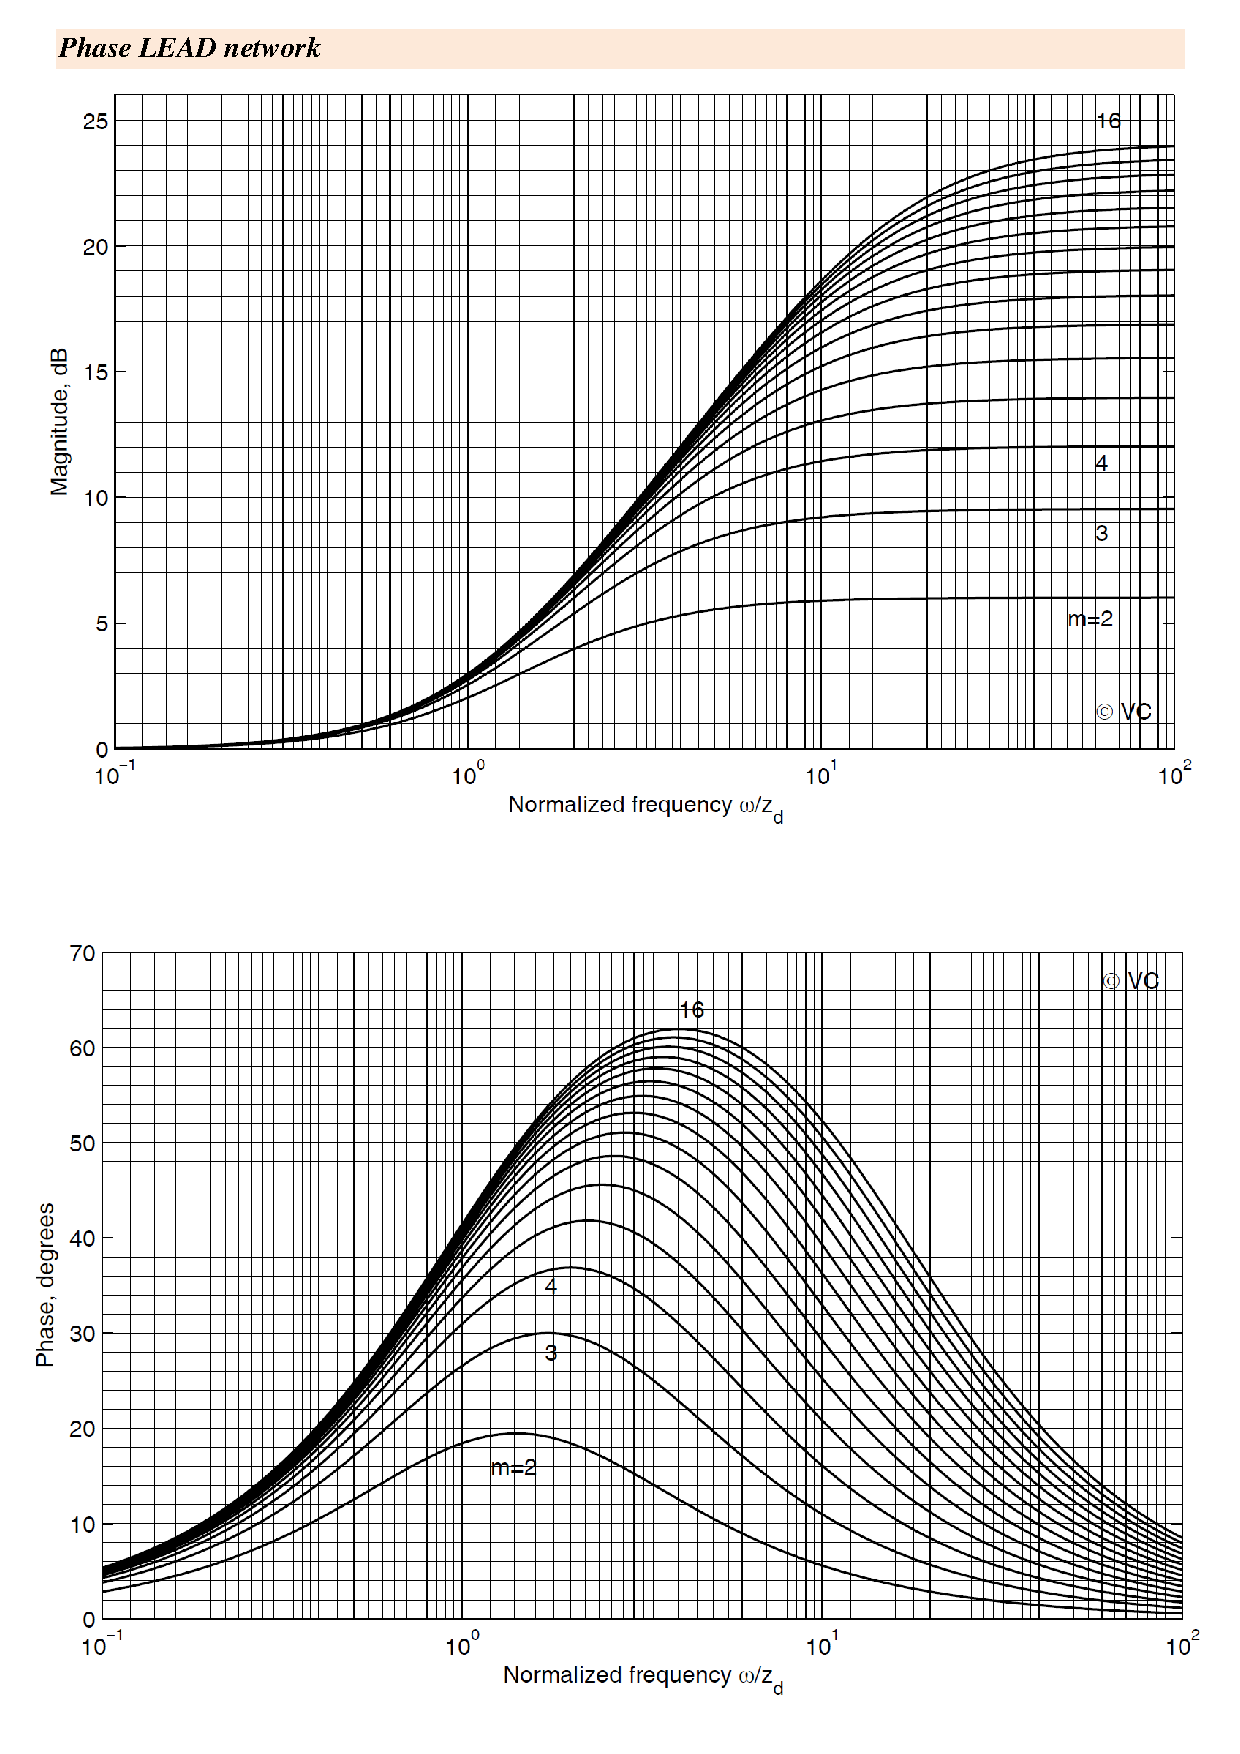
\includepdf[pages={-}]{reti_di_compensazione.pdf}

\end{document}
